\section{Model Validation}
\subsection{Units Consistency}
The units check validation is shown in Figure \ref{img:units}
\begin{figure}[H]
	\centering
    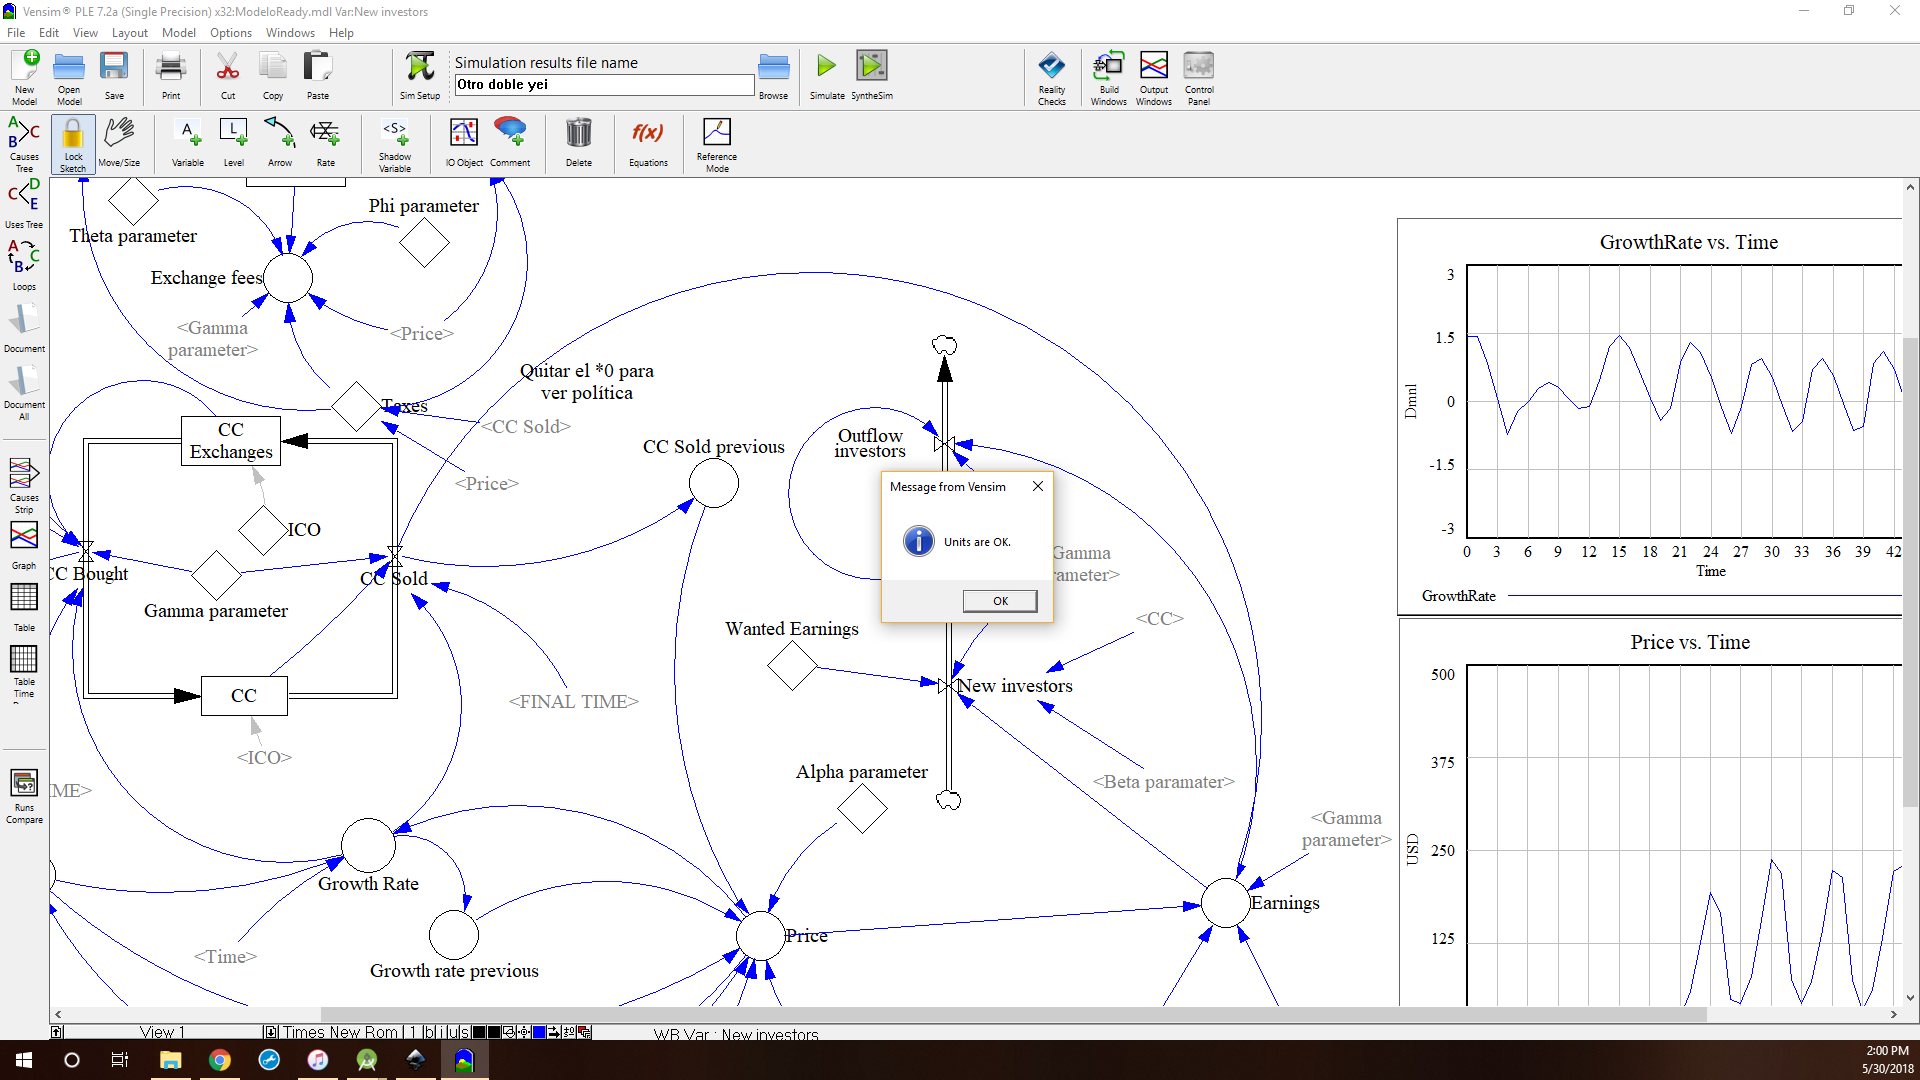
\includegraphics[scale=0.3]{files/Units.png}
    \caption{Units check in Vensim}
    \label{img:units}
\end{figure}
Though, it must be noted that the units check approval was achieved using some parameters, this proves that some of the equations proposed for the model are not the best options, even though they are consistent with whether the dependency was proportional or inversely proportional. 
\subsection{Stress Test}
	The variables selected for the stress test are CC Bought and New Investors. They were set as follows:
	\begin{multicols}{2}
    \begin{itemize}
    \item CCBought$=0$
    \columnbreak 
    \item NewInvestors$=0$
    \end{itemize}
		
	\end{multicols}
	
	\subsubsection{CC Bought}
		Setting the number of cryptocurrencies bought as zero, would imply an important drop in the price, this is shown in Figure \ref{img:extrprice}. This shows that the model behaves correctly after changing CCBought. 
        \begin{figure}[H]
        	\centering
            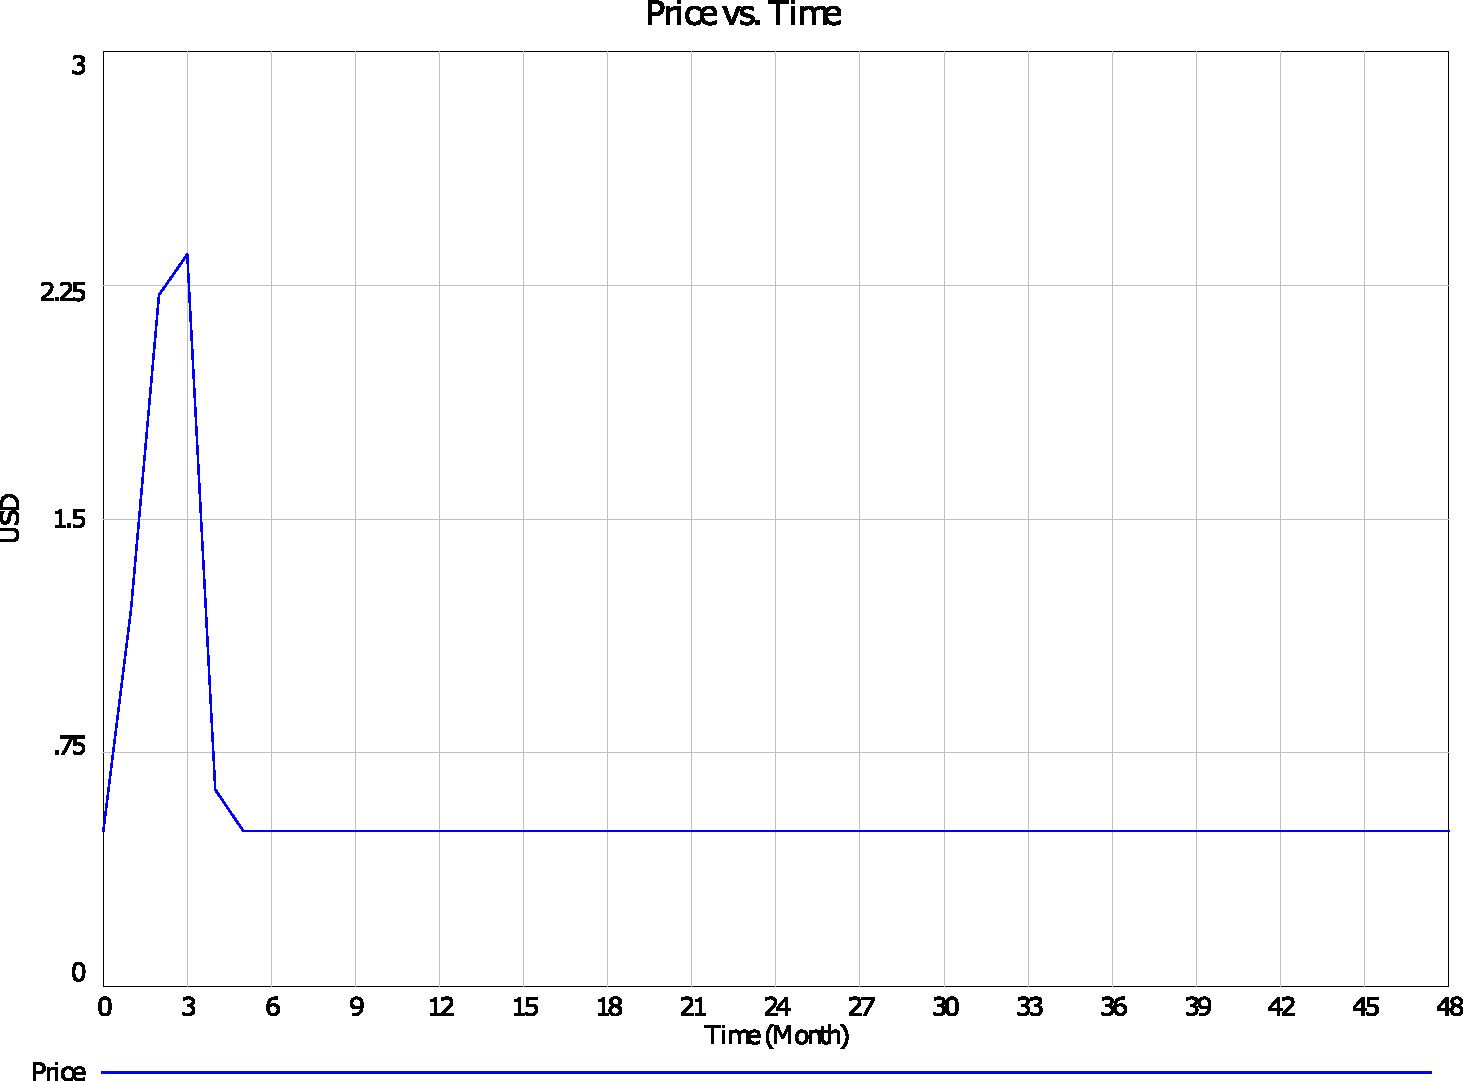
\includegraphics[scale=0.3]{files/ExtrPrice.pdf}
            \caption{Price after setting CCBought as zero.}
            \label{img:extrprice}
        \end{figure}
        On the other hand, it is important to note that the growth rate also behaves accordingly, as it is shown in Figure \ref{img:extrgrowth}. This is because it settles after a few months, which proves that it depends on the price change and it if it does not change, the growth rate will be constant.
        
        \begin{figure}[H]
        	\centering
            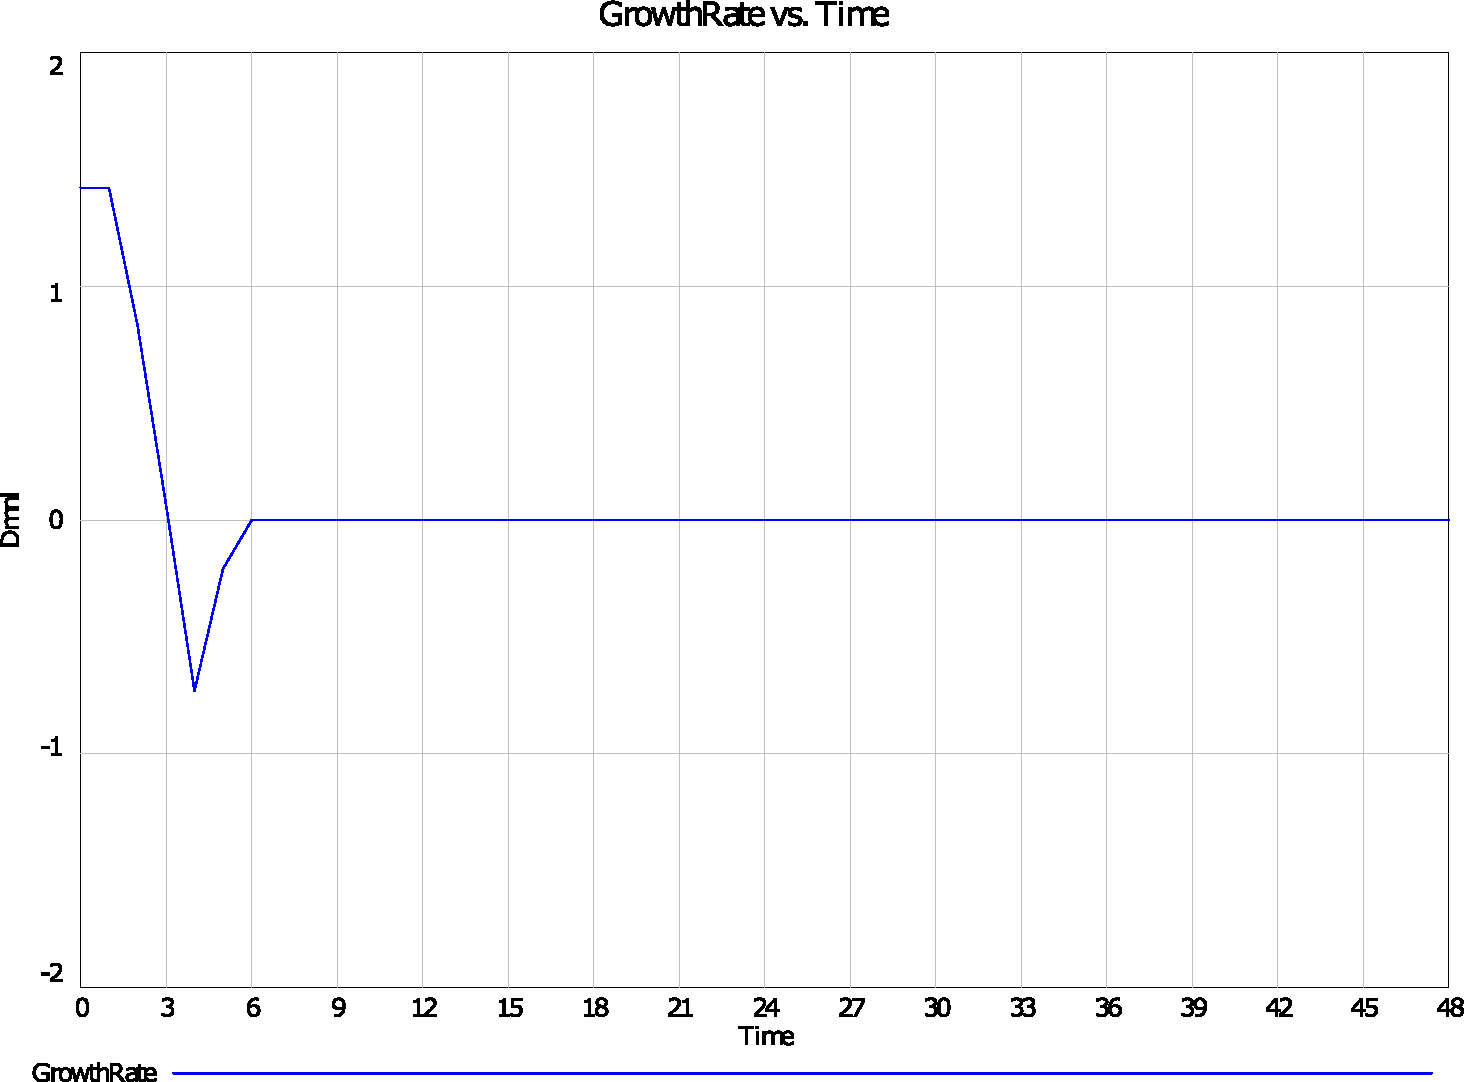
\includegraphics[scale=0.3]{files/ExtrCCBoughtGrowth.pdf}
            \caption{Growth rate behavior for CCBought as zero.}
            \label{img:extrgrowth}
        \end{figure}
        
	\subsubsection{New Investors}
    	Setting the number of new investors as zero, implies that there will not be new buyers and the market would, kind of, get stuck with the same people. As the cryptocurrency market needs people to invest and them being in a constant flow, the price of the CC would drop after a few months. This was achieved during this test, as shown in Figure \ref{img:extrinvprice}
        \begin{figure}[H]
        	\centering
            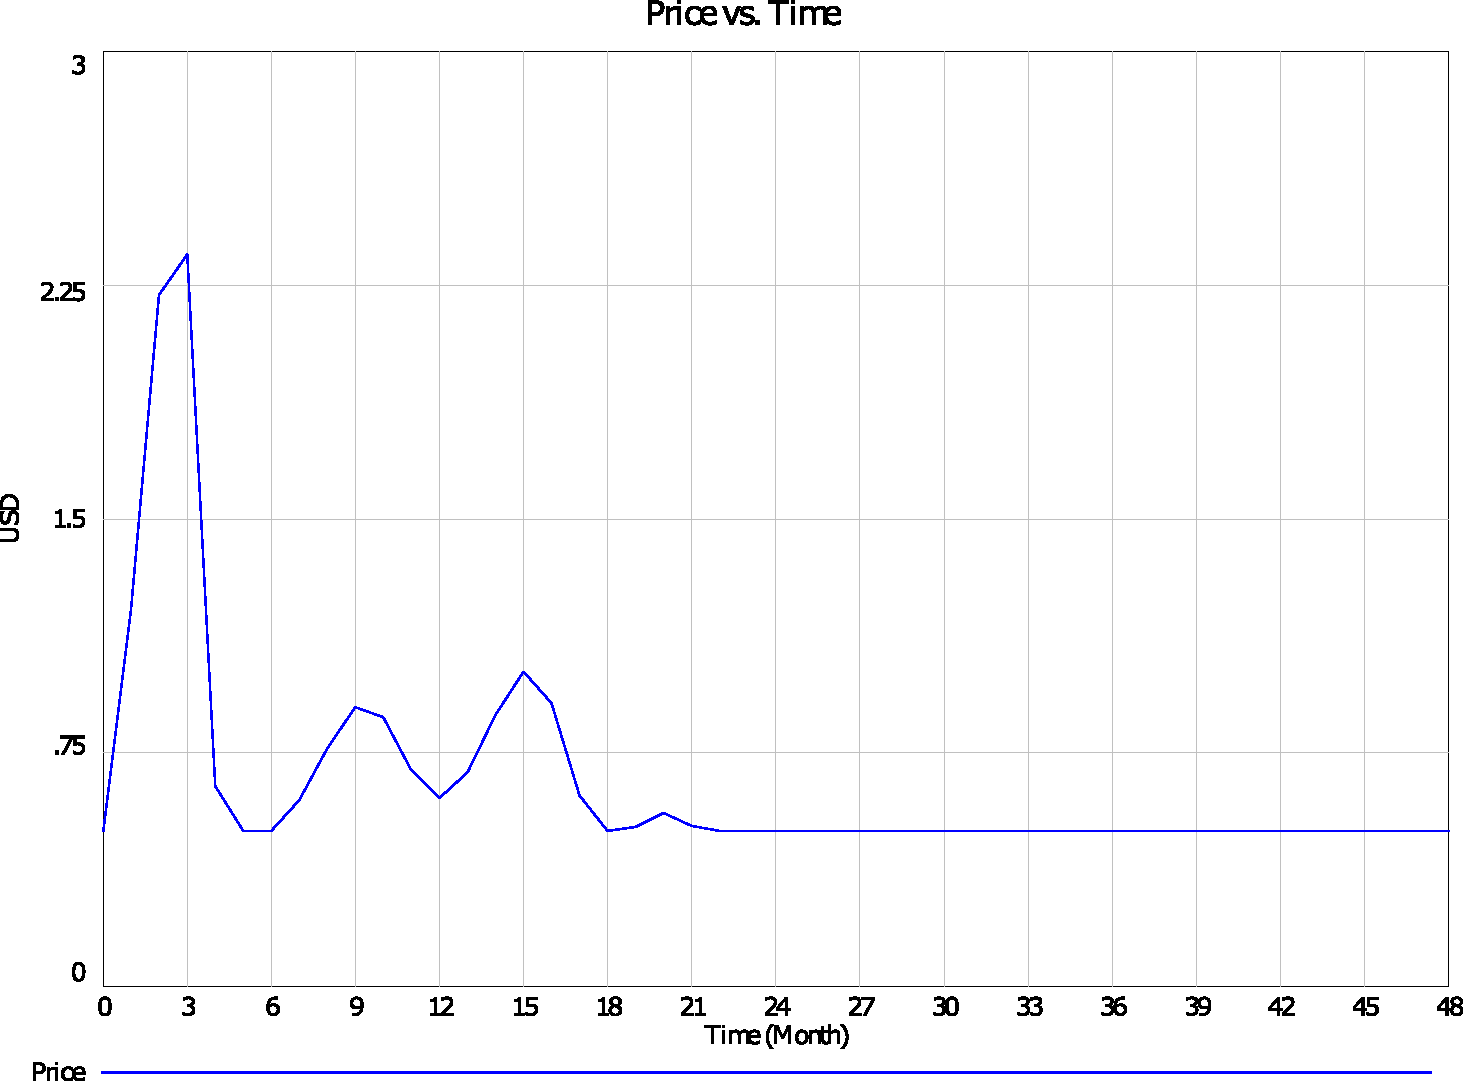
\includegraphics[scale=0.3]{files/ExtrInvestPrice.pdf}
            \caption{Results for price after setting the new investors as zero.}
            \label{img:extrinvprice}
		\end{figure}
        Same for the growth rate, which proves accordingly the behavior, shown in Figure \ref{img:extrinvgrowth}.
        \begin{figure}[H]
        	\centering
            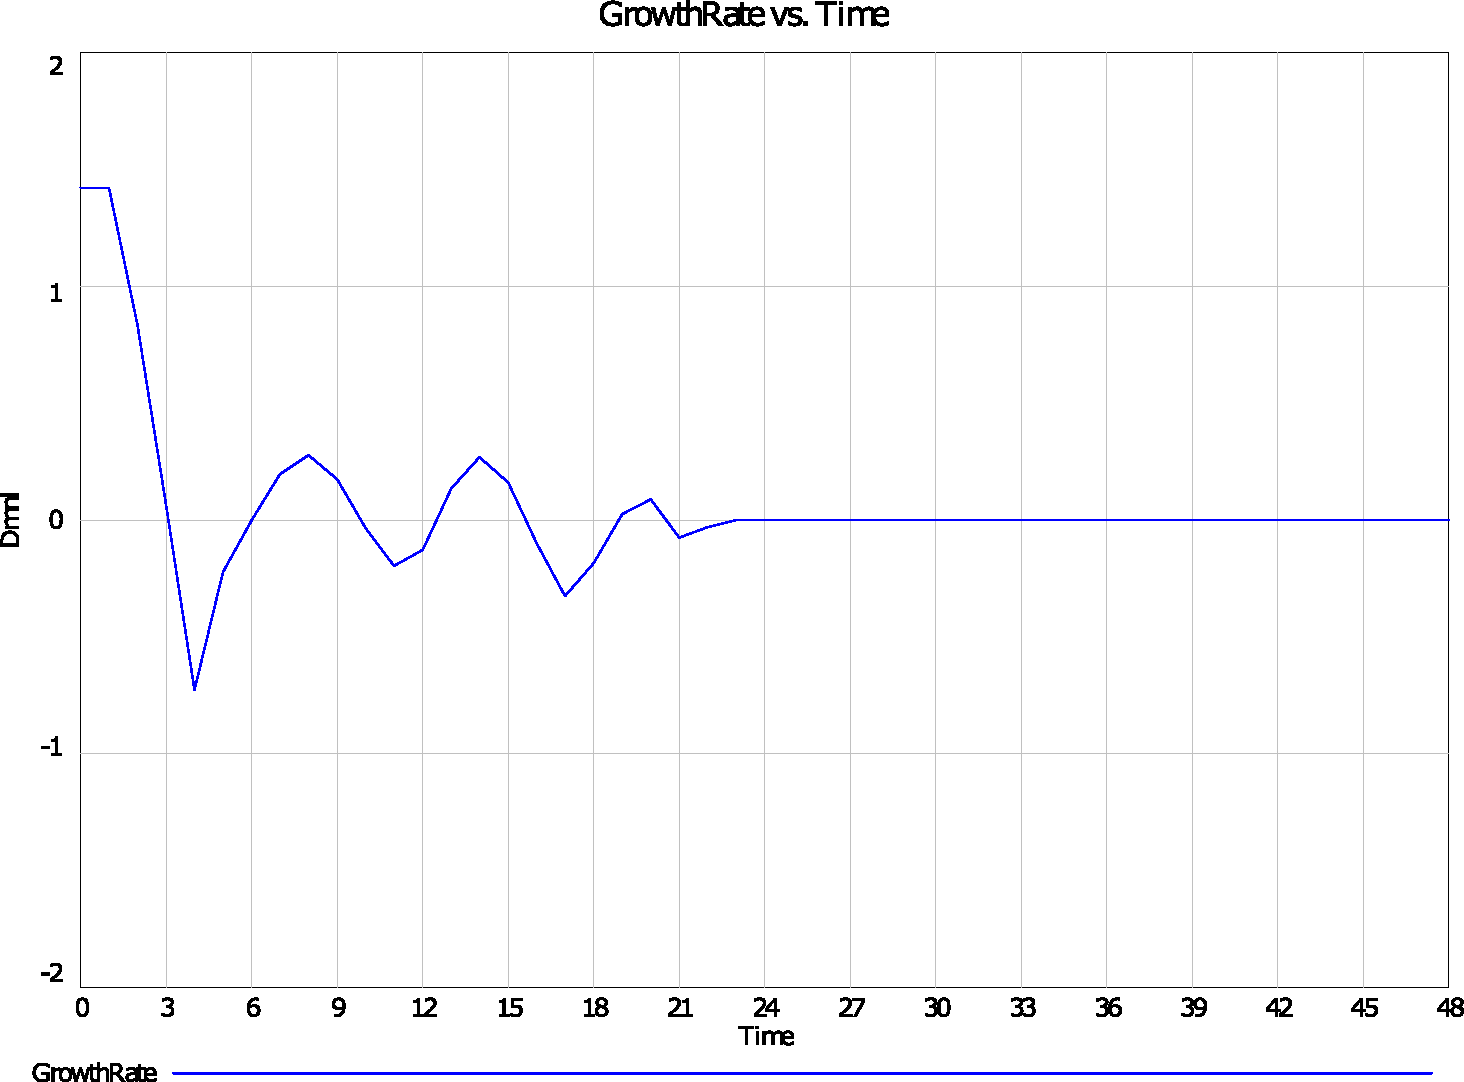
\includegraphics[scale=.3]{files/ExtrInvestGrowth.pdf}
            \caption{Results for Growth Rate for zero new investors.}
            \label{img:extrinvgrowth}
        \end{figure}
